\subsection{Encoding via ResNet50}
The learning curves as shown in Figure \ref{fig:resnet50_learning_curve} act in a very similar manner
as with the VGG19 models,
the difference that can be identified is the variation of the validation losses over the epochs.
Apart from that, the same starting and resulting loss is reached by the model,
without any overfitting or training problems.
The validation curve follows the training curve, supporting that the training dataset
is representative to the whole dataset.
It is to be noted that the training was done in different dataset split ups for all models.

\begin{figure}[H]
    \centering
    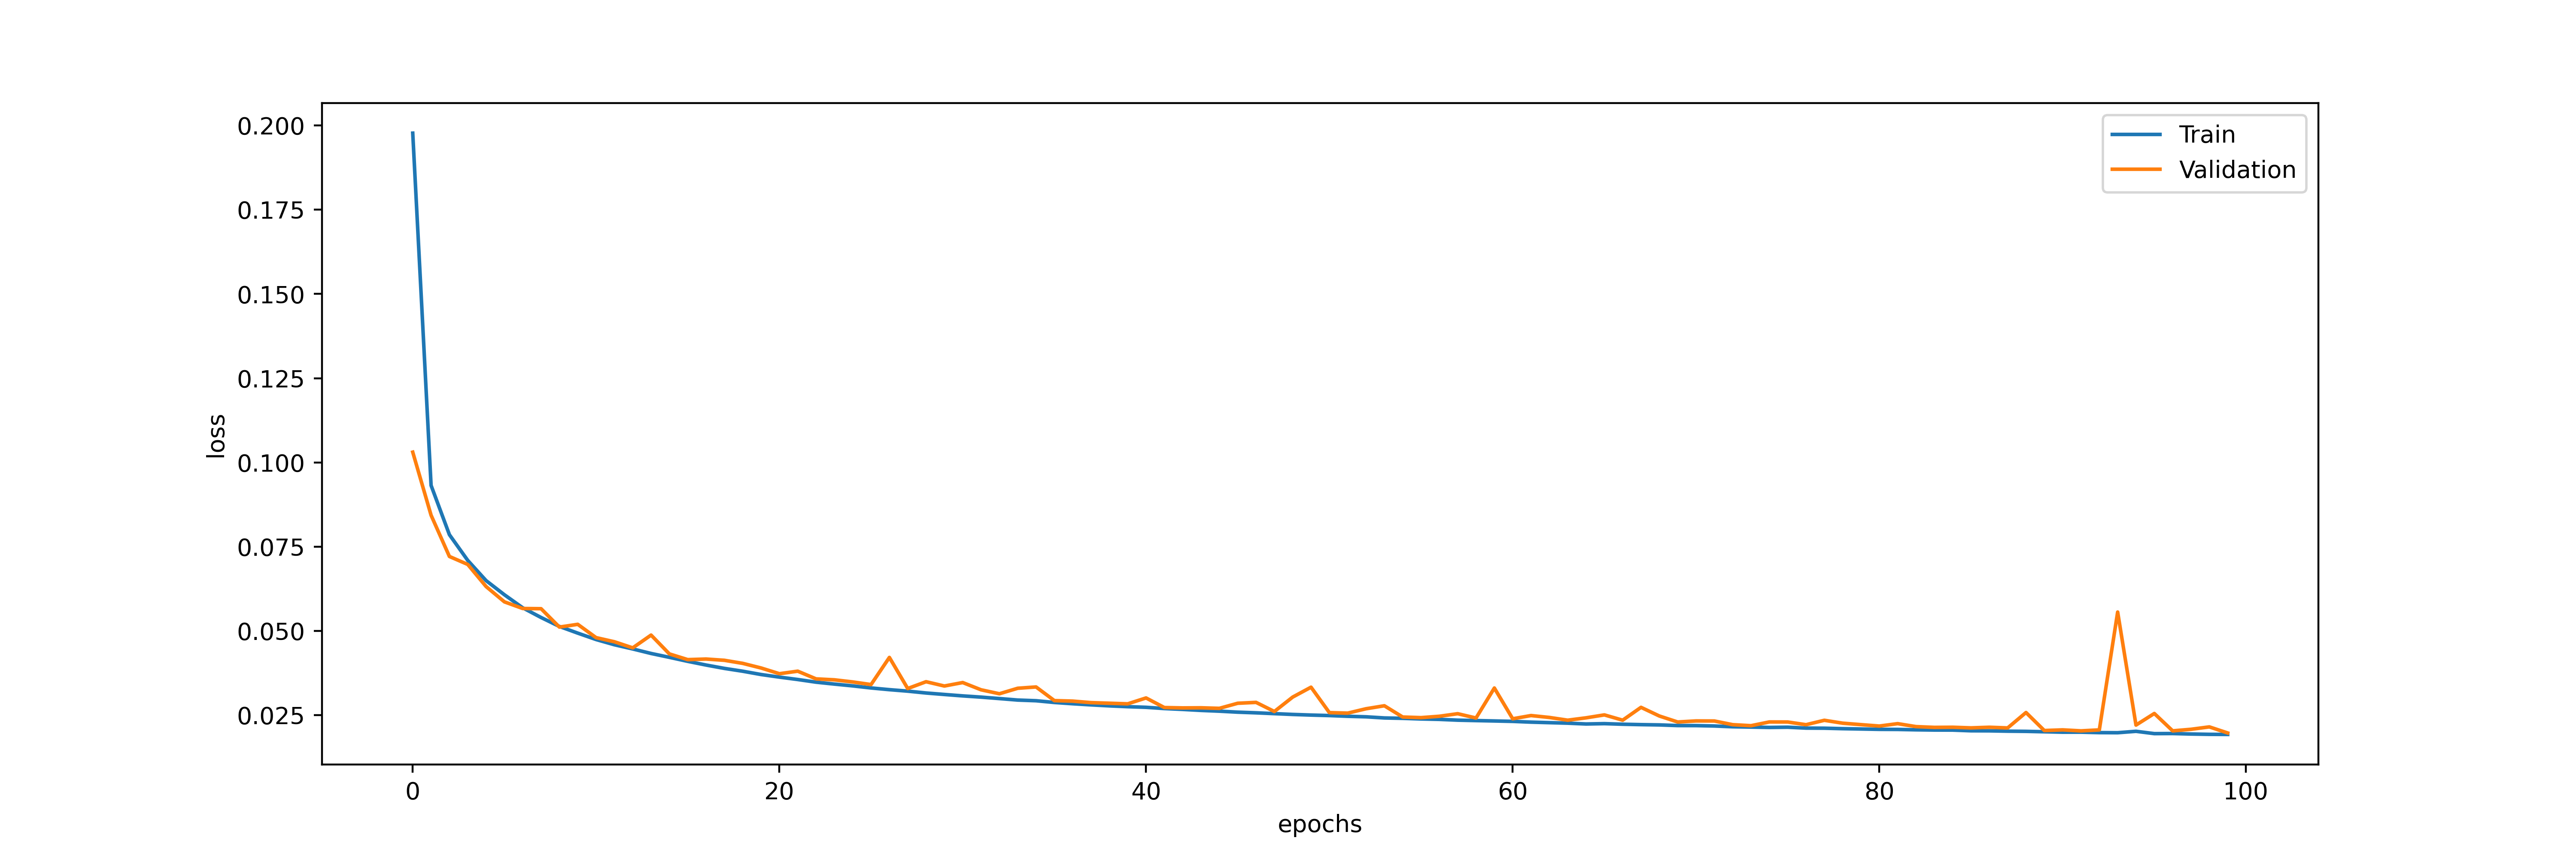
\includegraphics[width=\textwidth,trim={0 0 0 1cm},clip]{./results/resnet50_vgg19/20230514_213740_results.png}
    \caption{Learning curve of the ResNet50 Encoder}
    \label{fig:resnet50_learning_curve}
\end{figure}

The autoencoded images follow the same pattern as before, major features of the rail is regenerated,
the details are concentrating in the center or brighter parts of the images,
the main edge of the running surface of the rail and the side surface both can be identified.
The representation of the ballast rocks also present.
These are presented on Figure \ref{fig:resnet50_examples}.
It can be concluded that the model learned to encode the images to feature vectors and then the
decoding is also successful, however it has to be noted that the resulting image is far from complete.

\begin{figure}[H]
    \centering
    \begin{subfigure}{\textwidth}
        \centering
        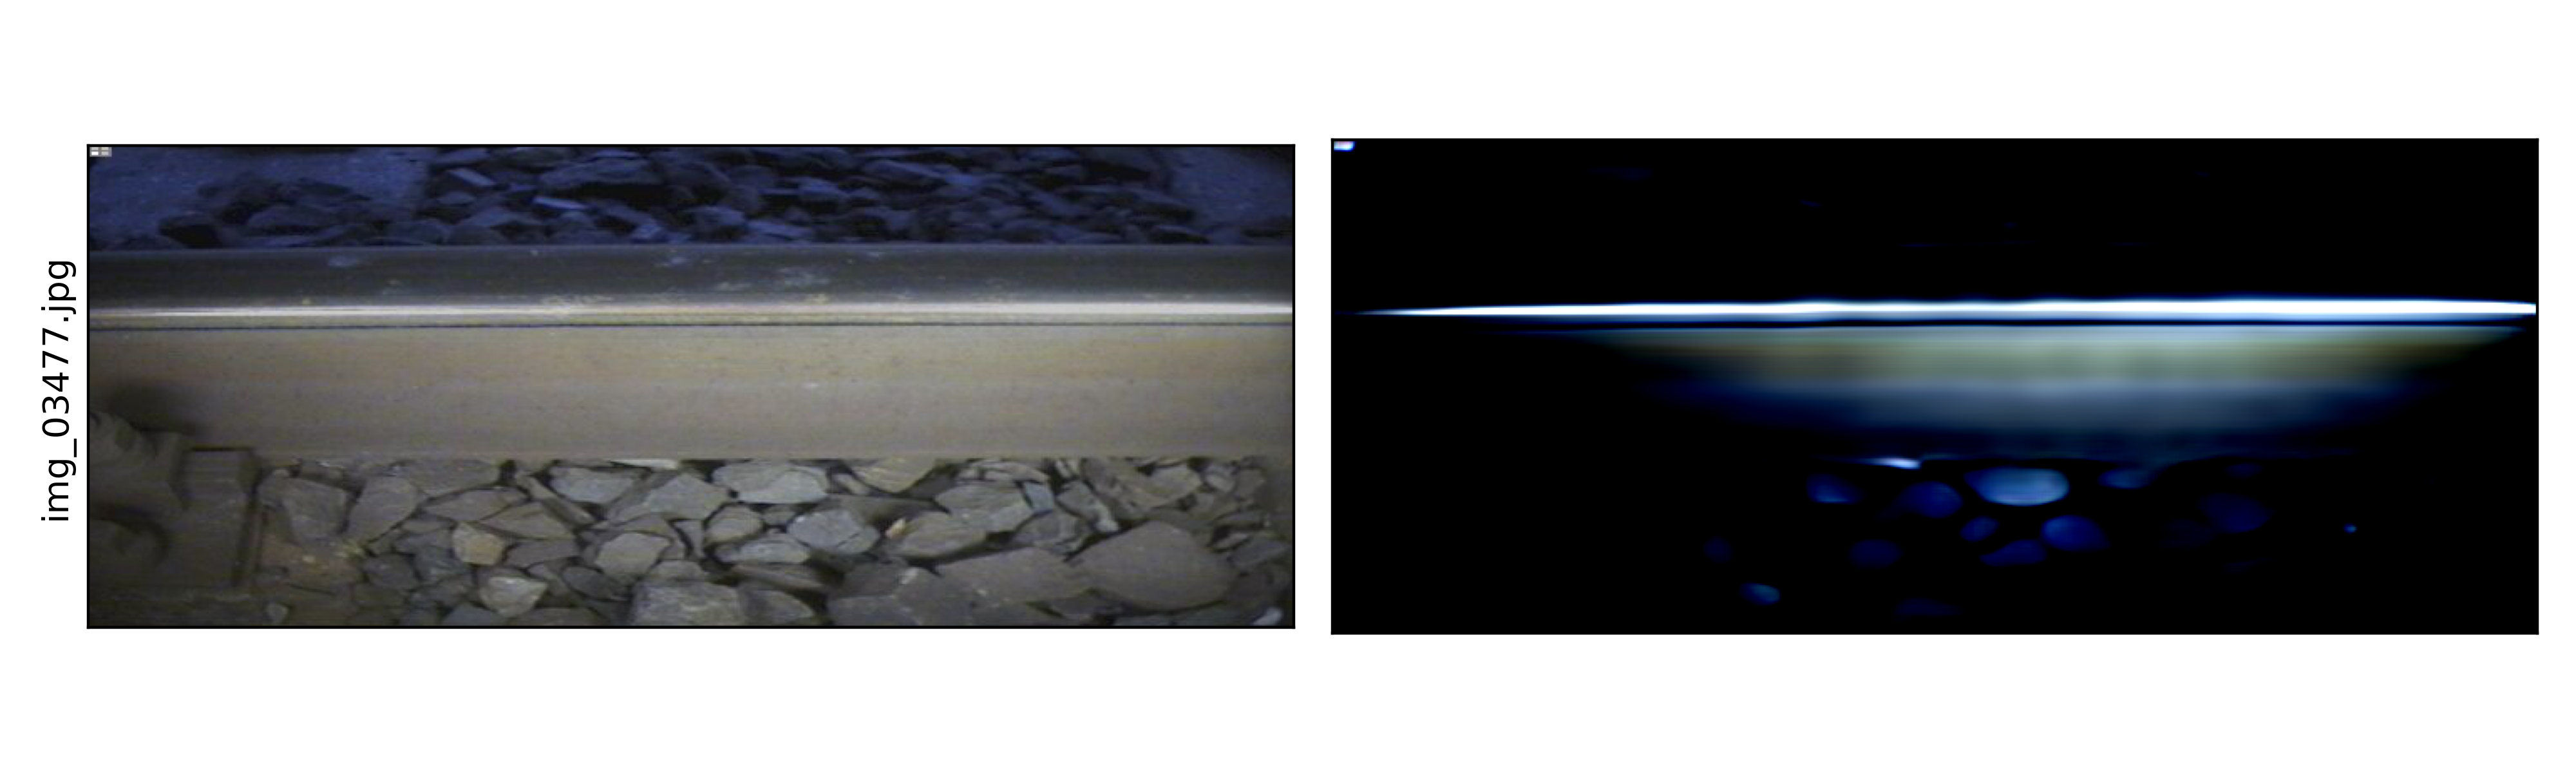
\includegraphics[width=0.9\textwidth,trim={0 1cm 0 1cm},clip]{./results/resnet50_vgg19/20230514_213740_predict_0.png}
    \end{subfigure}
    \begin{subfigure}{\textwidth}
        \centering
        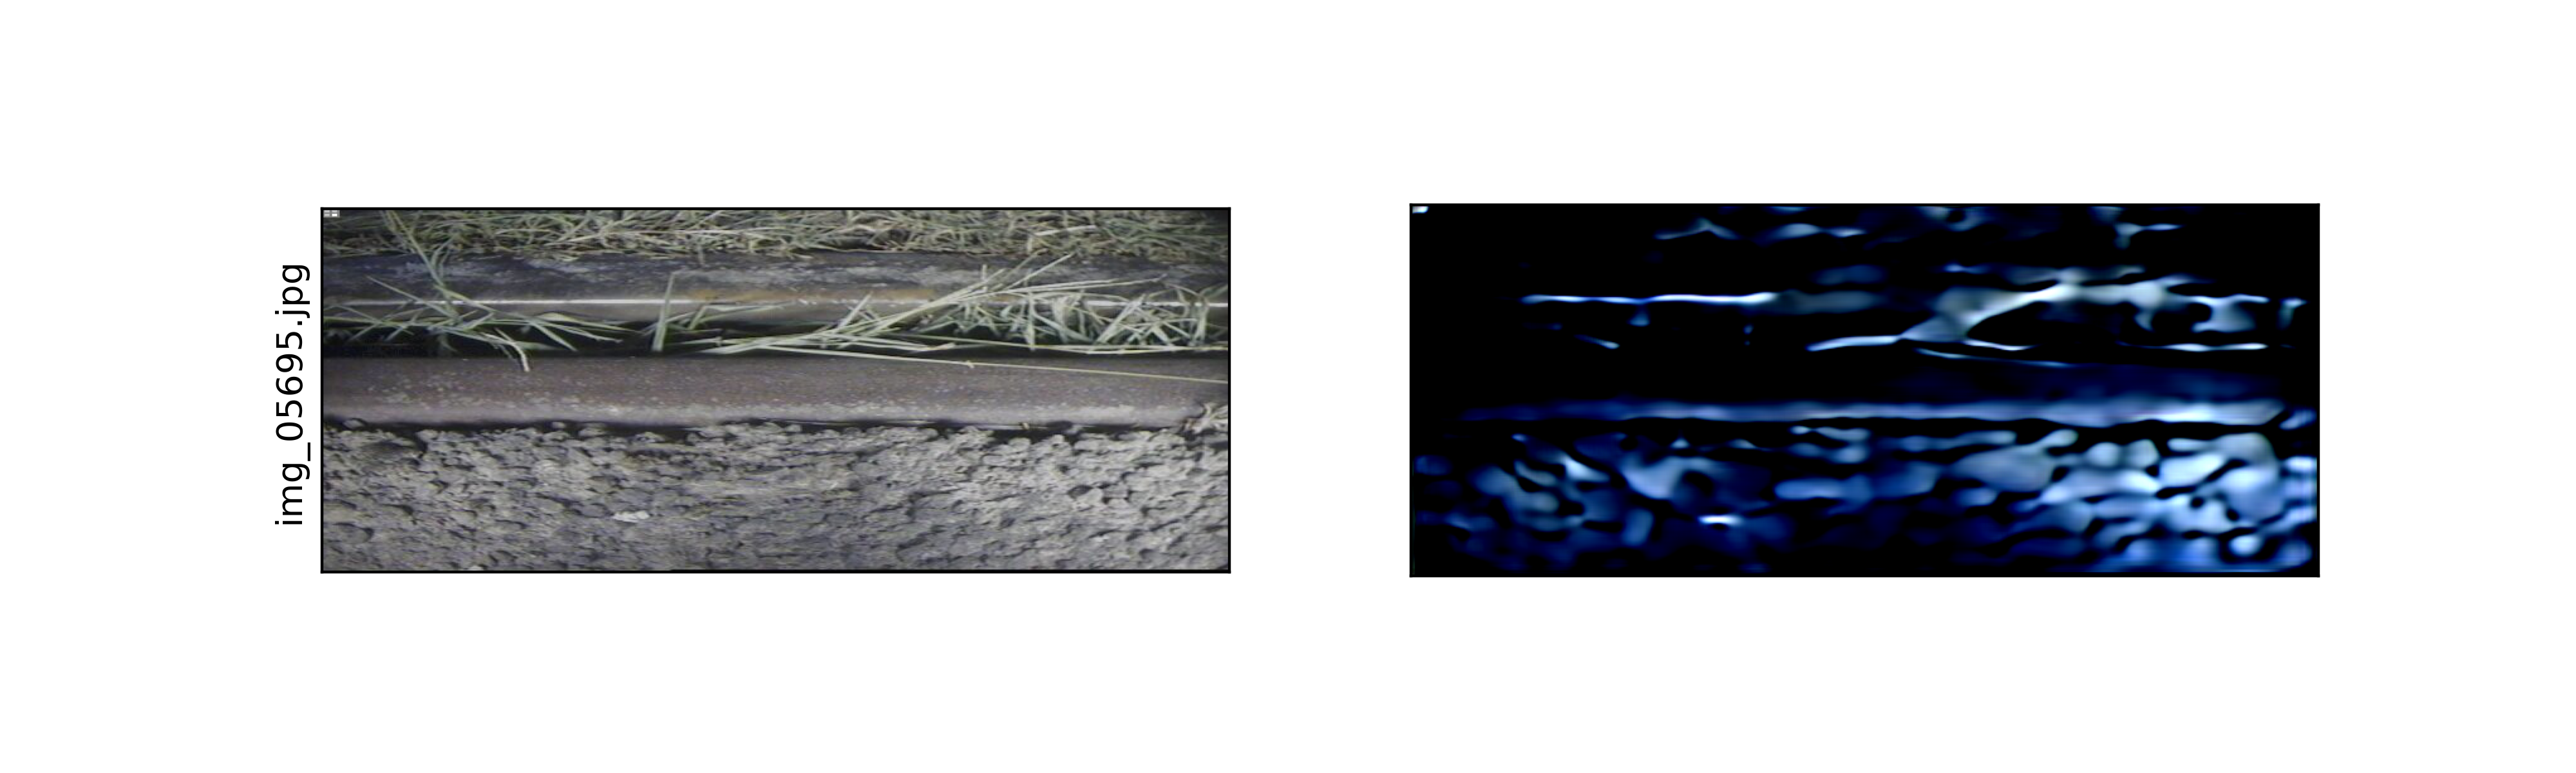
\includegraphics[width=0.9\textwidth,trim={0 1cm 0 1cm},clip]{./results/resnet50_vgg19/20230514_213740_predict_1.png}
    \end{subfigure}
    \begin{subfigure}{\textwidth}
        \centering
        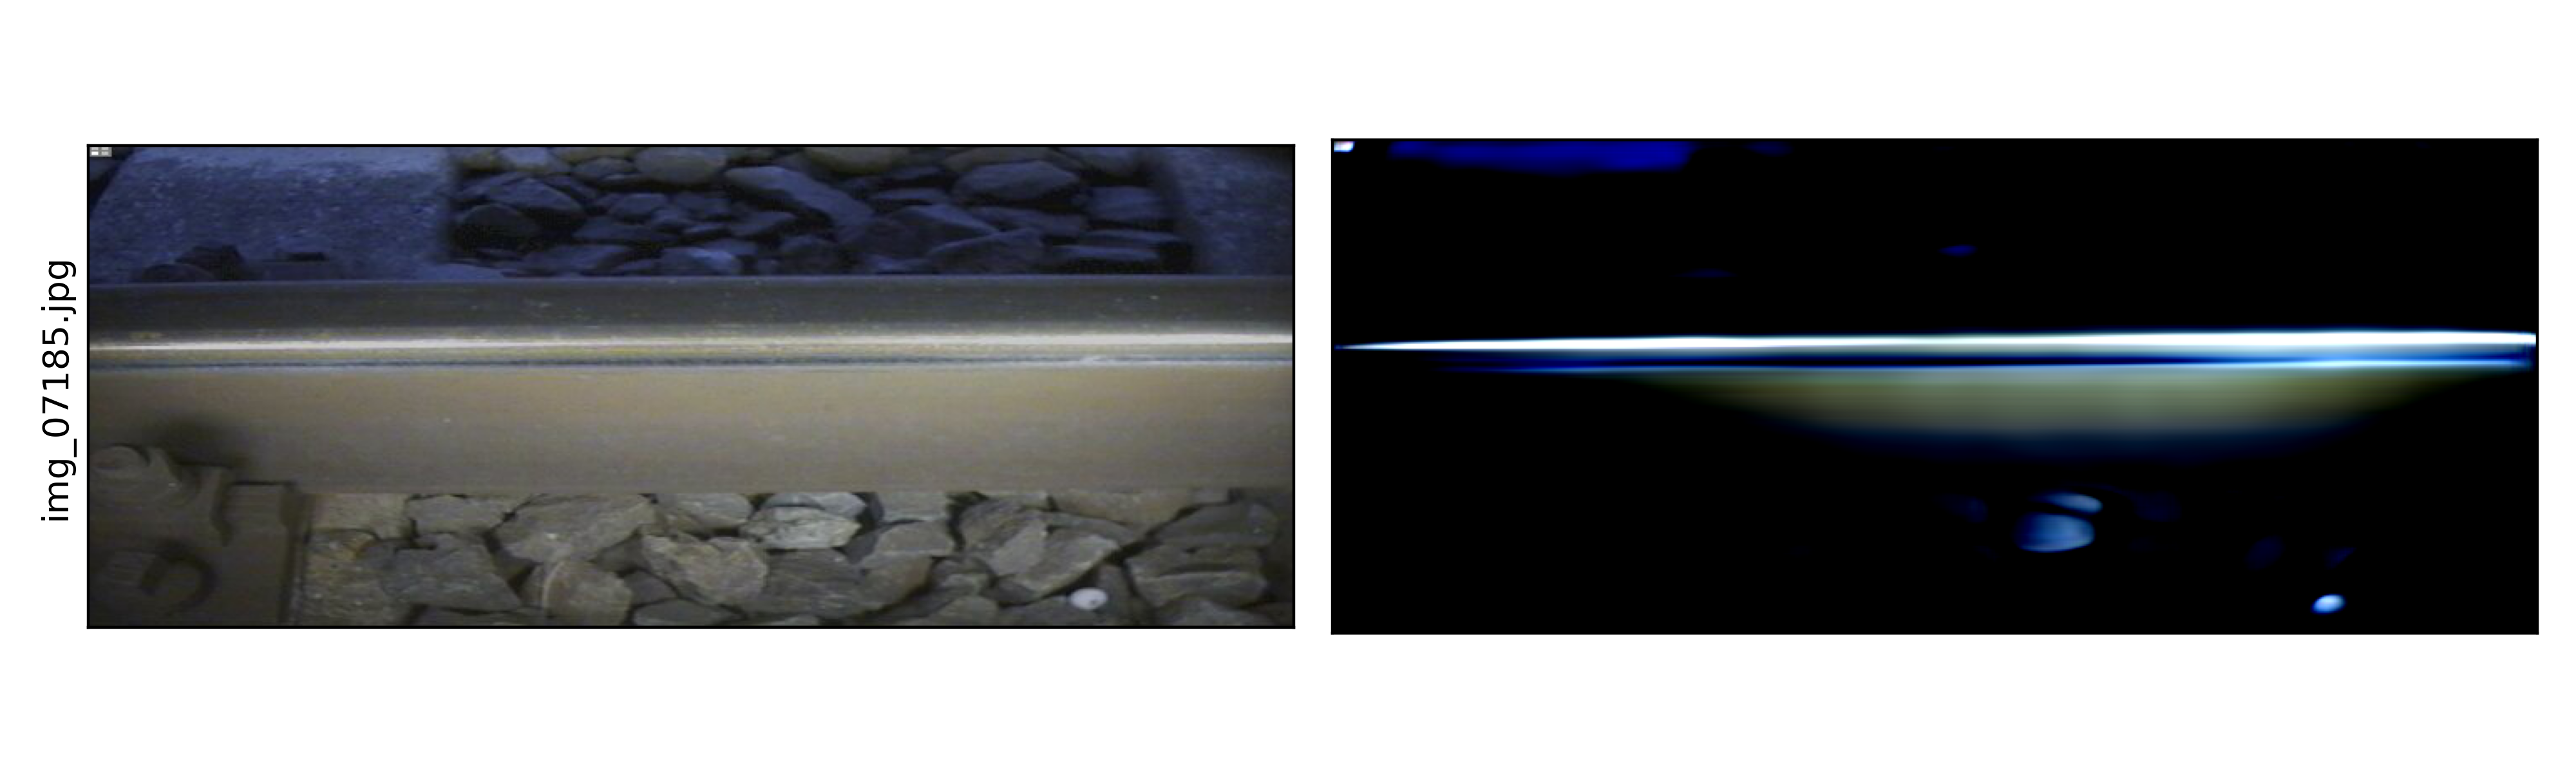
\includegraphics[width=0.9\textwidth,trim={0 1cm 0 1cm},clip]{./results/resnet50_vgg19/20230514_213740_predict_2.png}
    \end{subfigure}
    \caption{Predicted images in case of ResNet50 Encoder}
    \label{fig:resnet50_examples}
\end{figure}

The PCA / t-SNE visualization shows a little enhancement in the behavior of the model
on Figure \ref{fig:resnet50_pca}.
The outliers of the input images are encoded in a way that they tend to separate from the
major \emph{normal} cluster, even the ones that remained in this cluster are closer to the boundary
as shown on the top right part of the encoded sub-figure.
Even it can be seen that this region or the boundary is \emph{opening up} and the \emph{normal}
images do not encompass these outliers so much.
The bottom right concentration of the outliers are separating clearly with this model,
as seen with the other models as well.
The decoded images retain the clustering in a strict manner, compared to the distribution of the
outliers on the input visualization, the decoded outliers form a more closed cluster.
Some outliers (that usually have low loss values compared to the other anomalies) still
remain inside the \emph{normal} cluster through the whole model.

\begin{figure}[H]
    \centering
    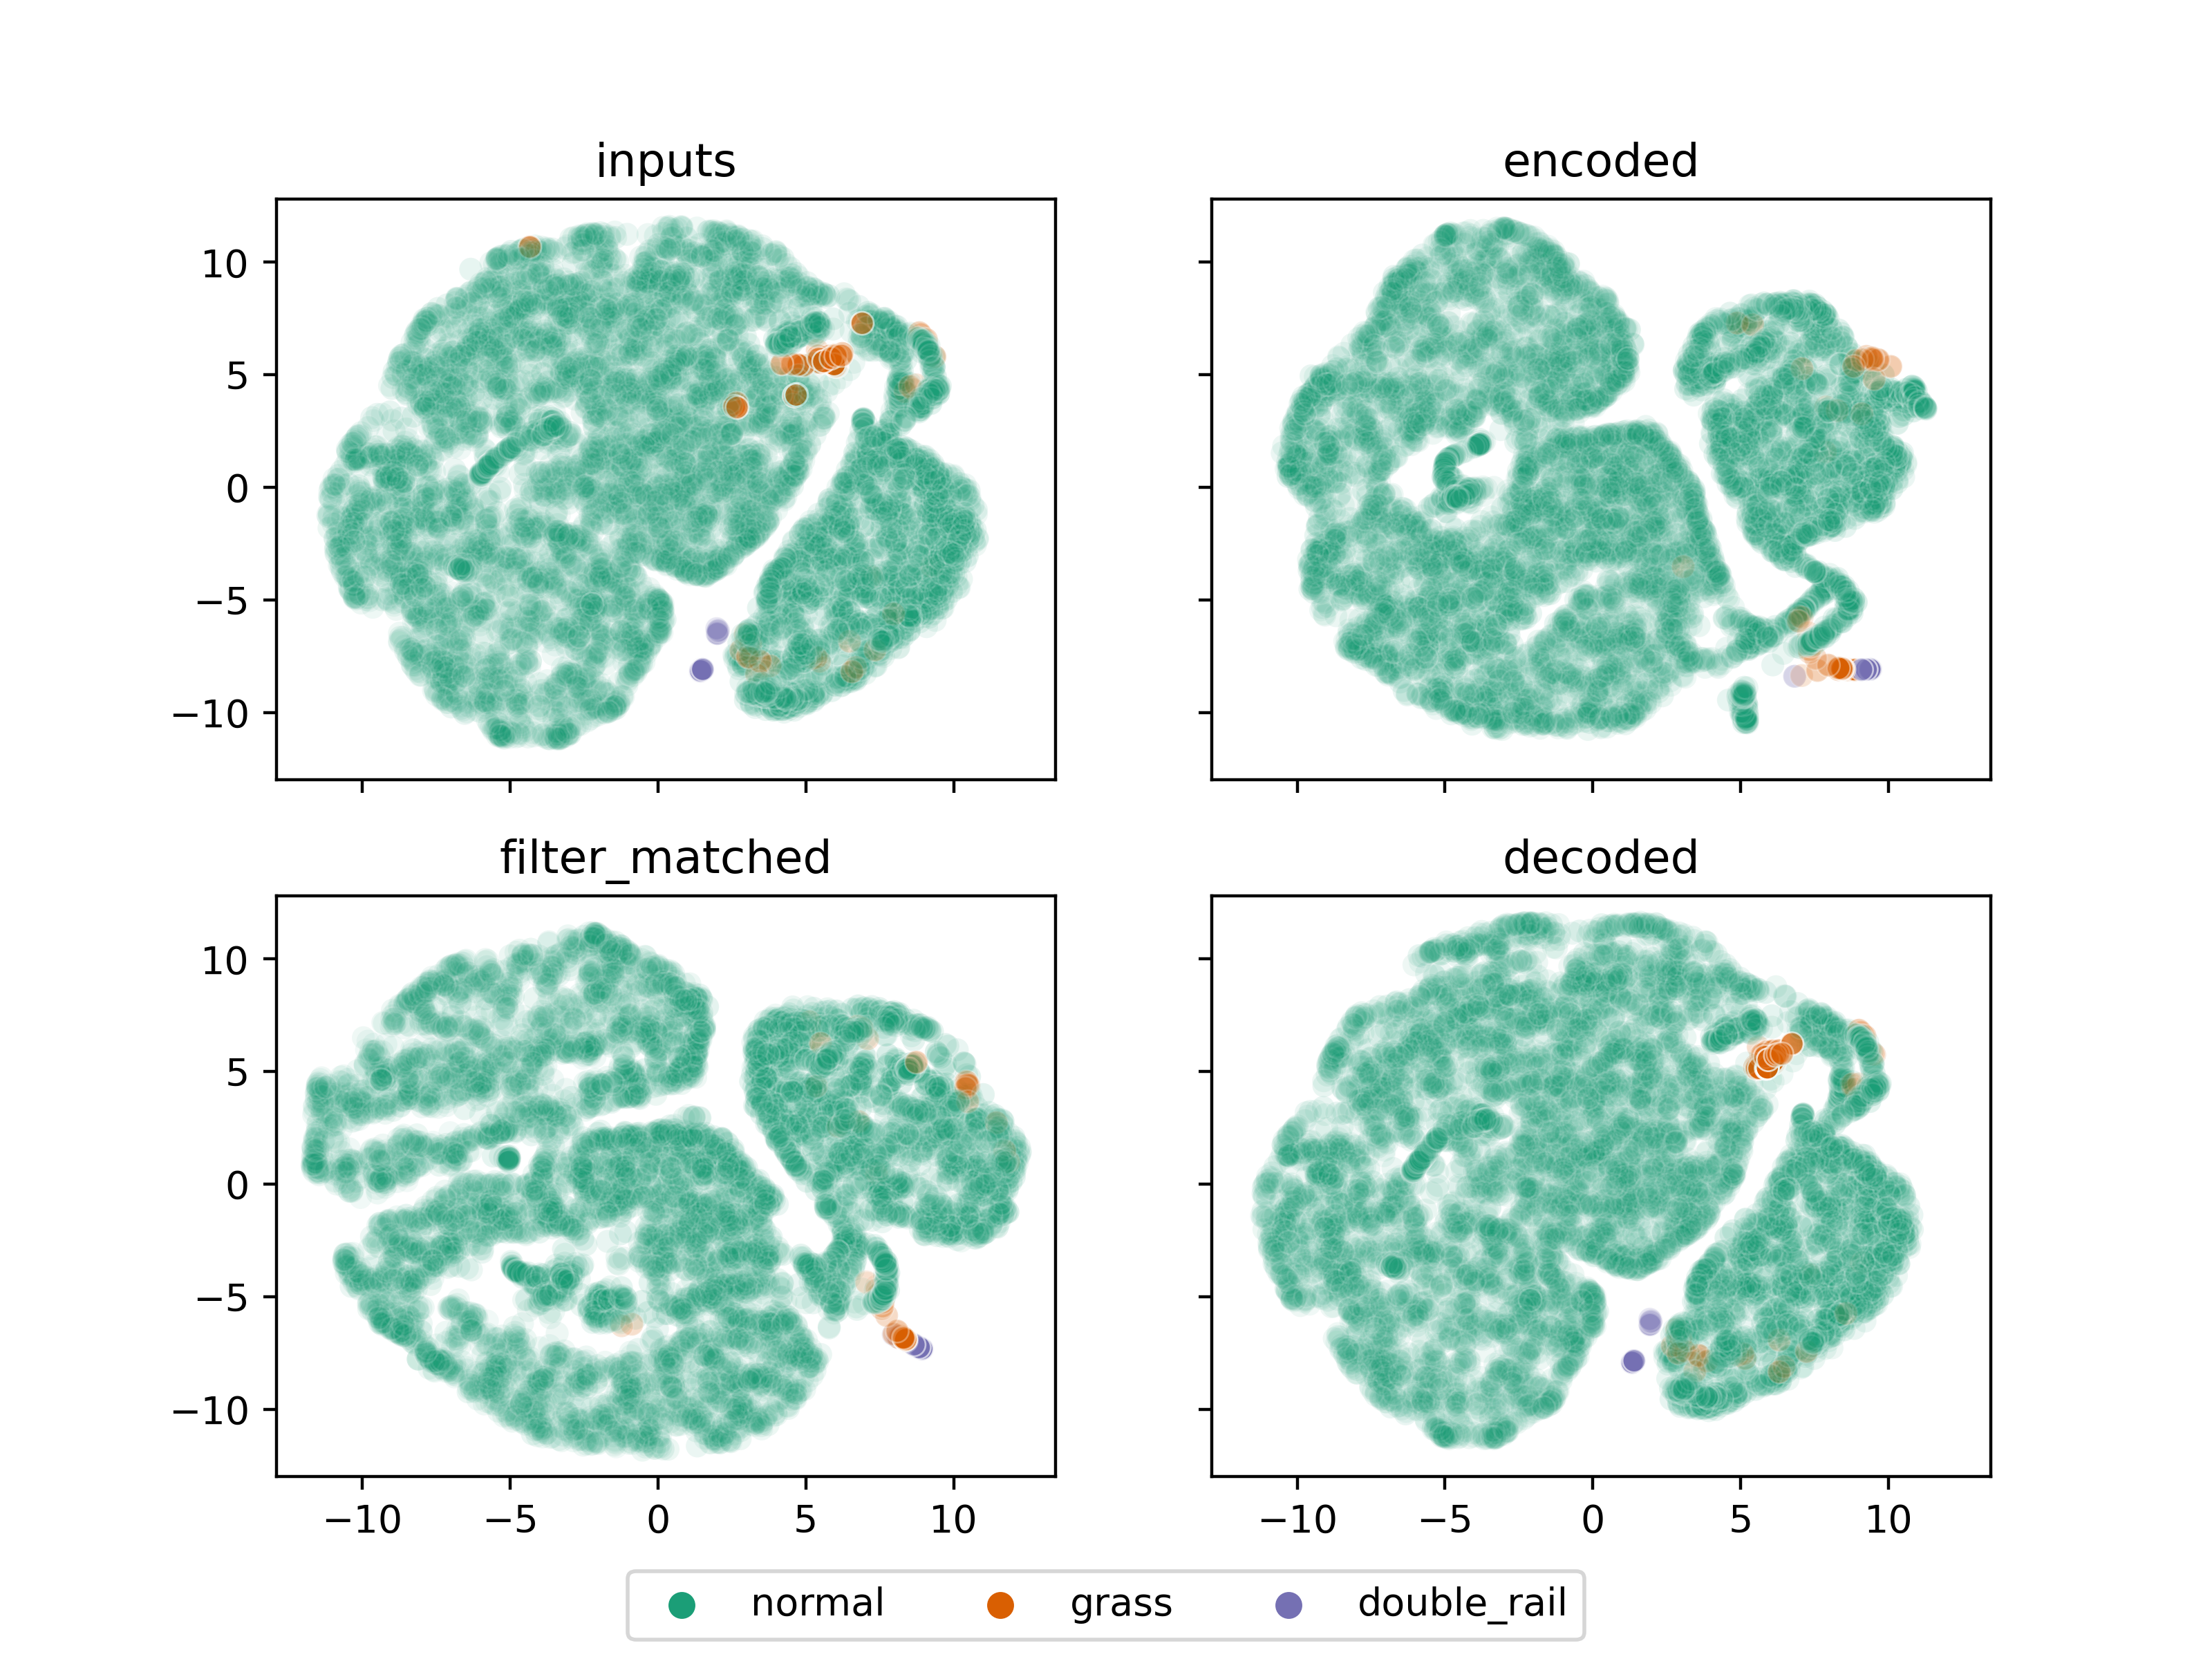
\includegraphics[width=0.8\textwidth,trim={0 0 0 1cm},clip]{./results/resnet50_vgg19/20230514_213740_feature_vectors_1.png}
    \caption{PCA / t-SNE visualization of the ResNet50 Encoder}
    \label{fig:resnet50_pca}
\end{figure}

The loss values depict the same variation over the images as seen for the VGG models,
depicted on Figure \ref{fig:resnet50_loss}.
The majority of the outliers can be easily identified, although not all of them have a high loss value
and some images with high loss values belong to the \emph{normal} rail class.
The loss values do not indicate a difference between the models seen so far.

\begin{figure}[H]
    \centering
    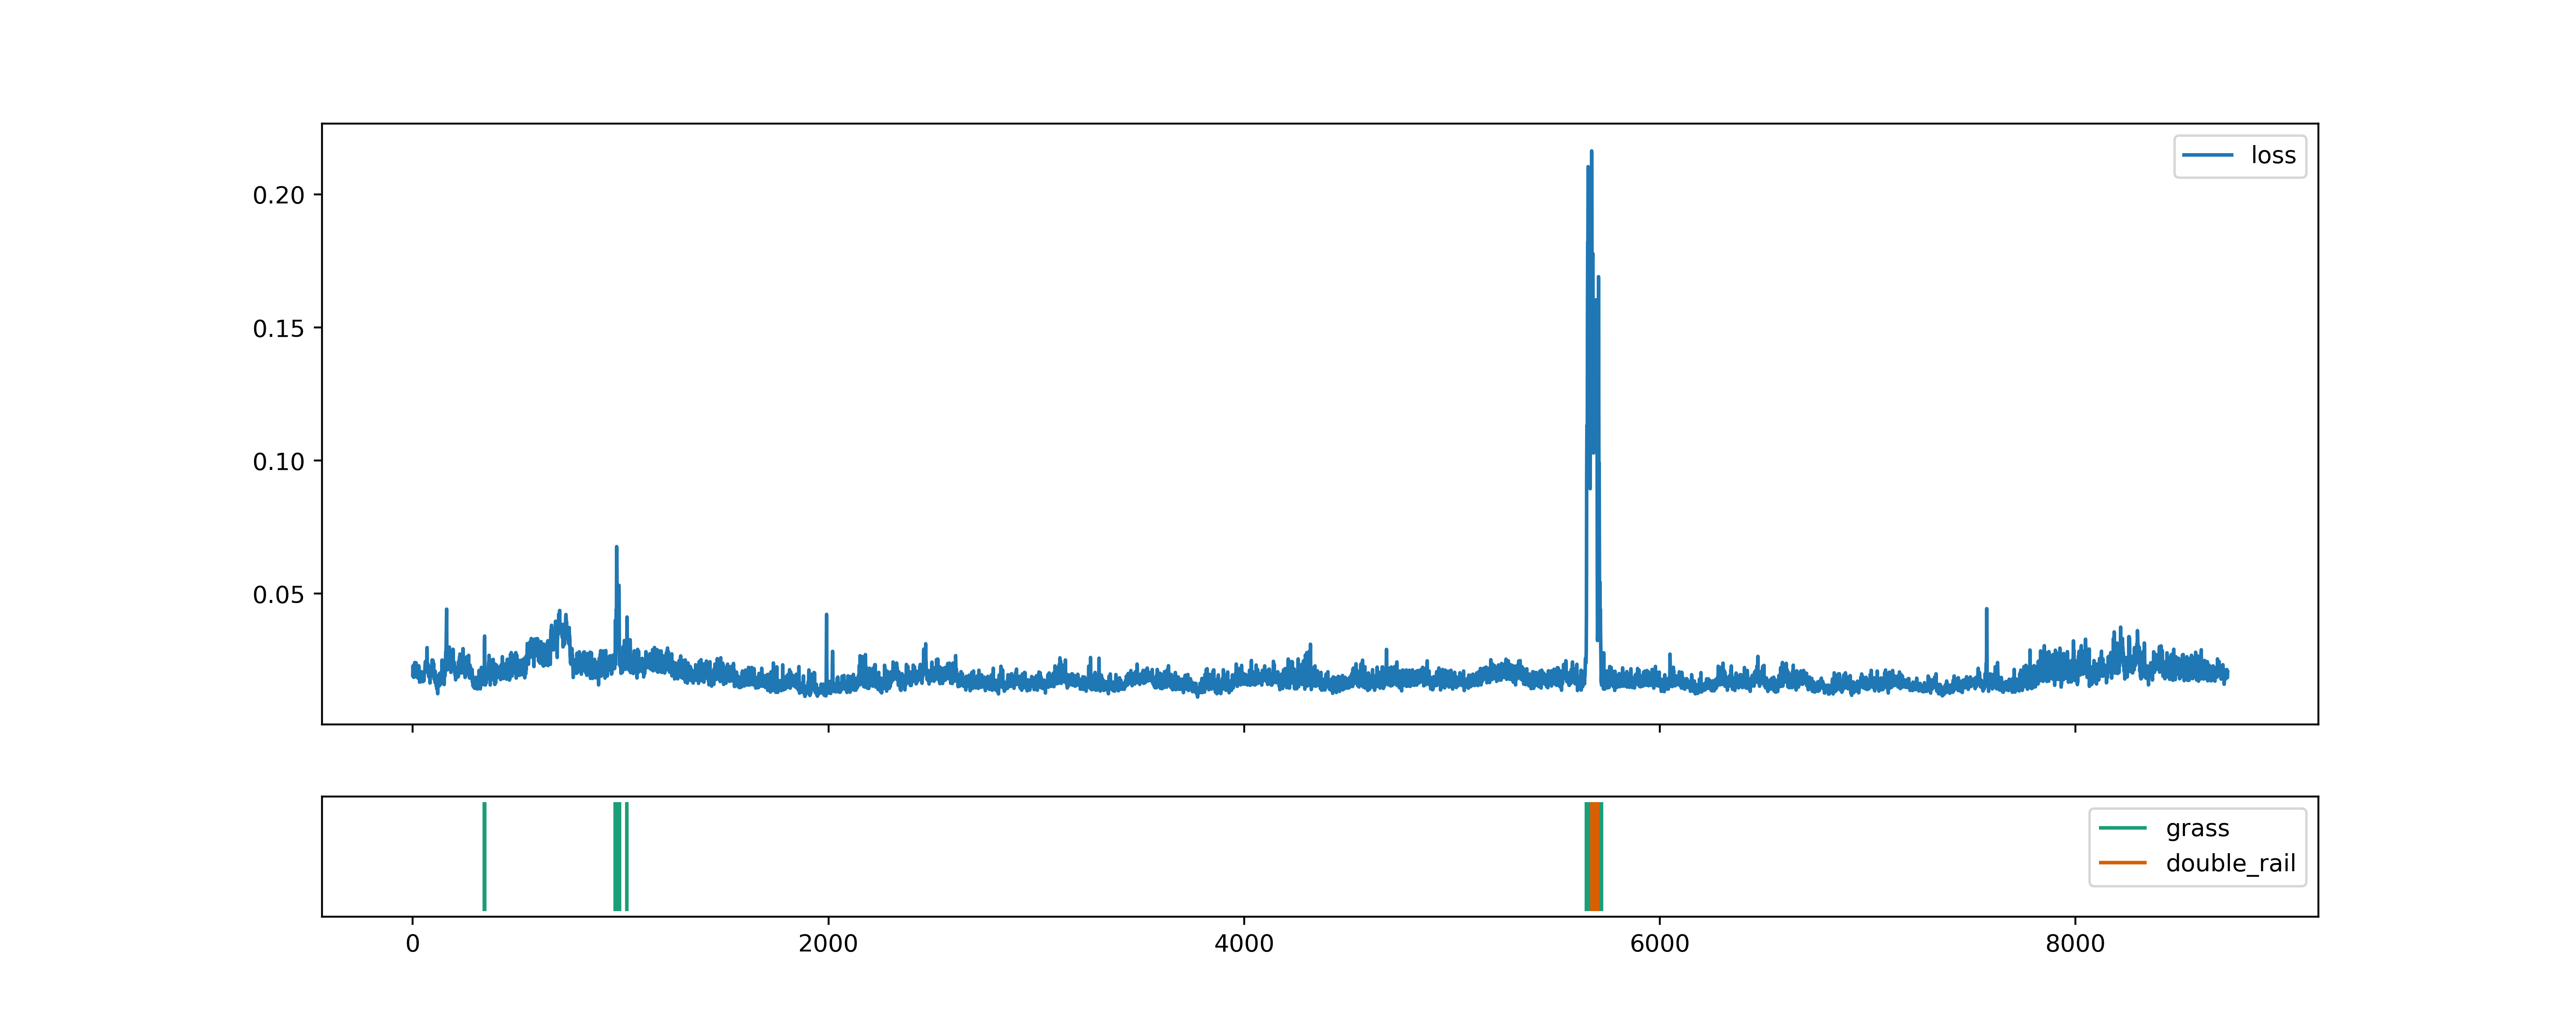
\includegraphics[width=\textwidth,trim={0 1cm 0 1cm},clip]{./results/resnet50_vgg19/20230514_213740_feature_vectors_loss.png}
    \caption{Loss values of the dataset with ResNet50 encoding}
    \label{fig:resnet50_loss}
\end{figure}

The classification metrics stay between the VGG19 models with and without batch normalization.
The confusion matrices can be seen on Figure \ref{fig:resnet50_cm}.
The loss-based approach delivers the same performance as the threshold still too conservative,
approximately \small \sfrac{2}{3} of the true positives identified correctly.
The Isolation Forest algorithm identifies true positives in higher rate than the VGG19 without
batch normalization, however the false positives remain on the level of a pure VGG19 model.

\begin{figure}[H]
    \centering
    \begin{subfigure}{0.4\textwidth}
        \centering
        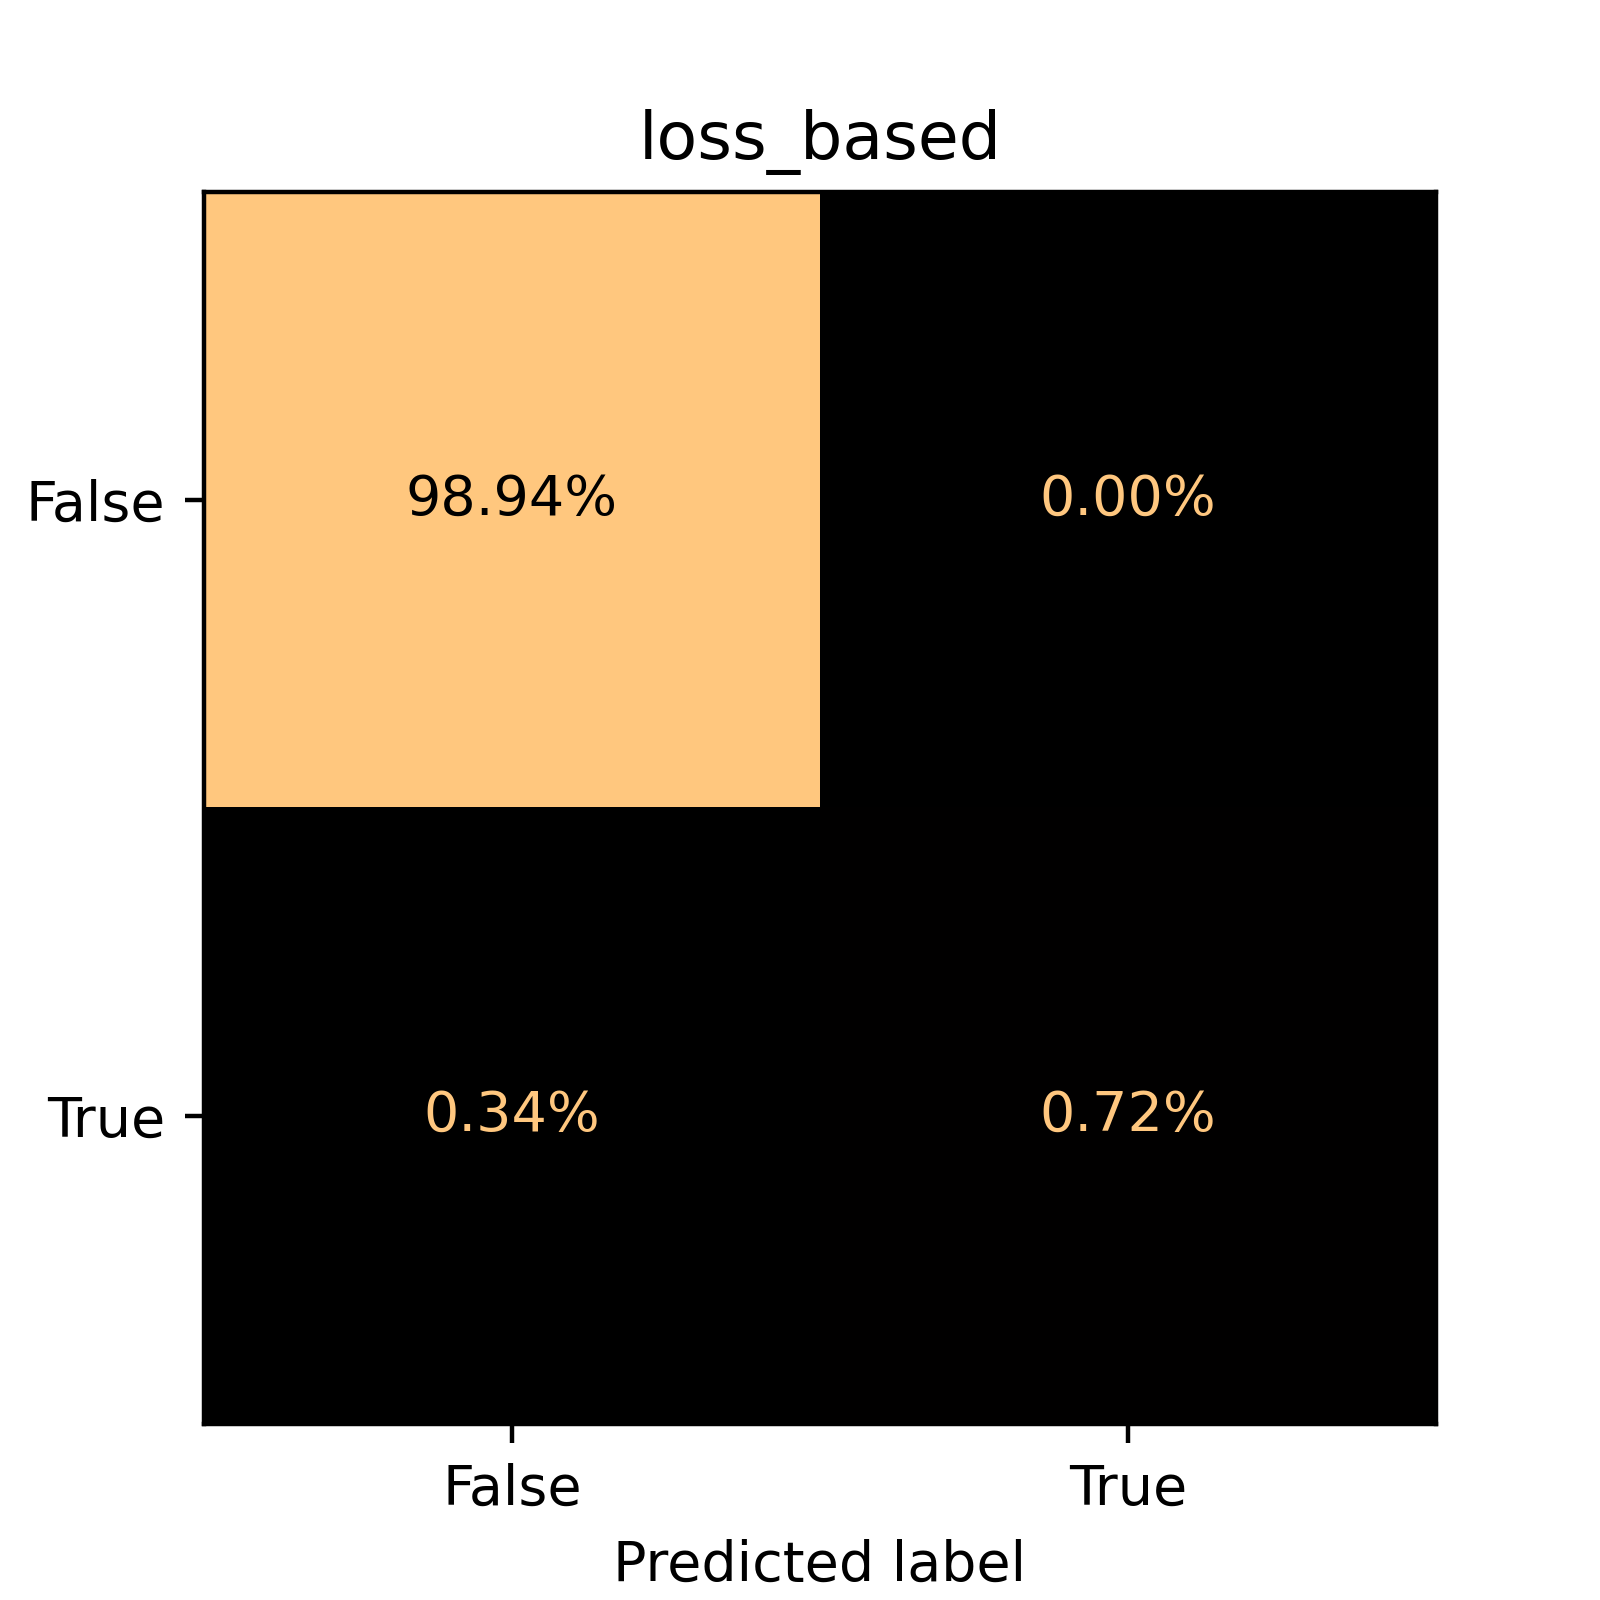
\includegraphics[width=\textwidth]{./results/resnet50_vgg19/20230514_213740_loss_based_cm.png}
    \end{subfigure}
    \begin{subfigure}{0.4\textwidth}
        \centering
        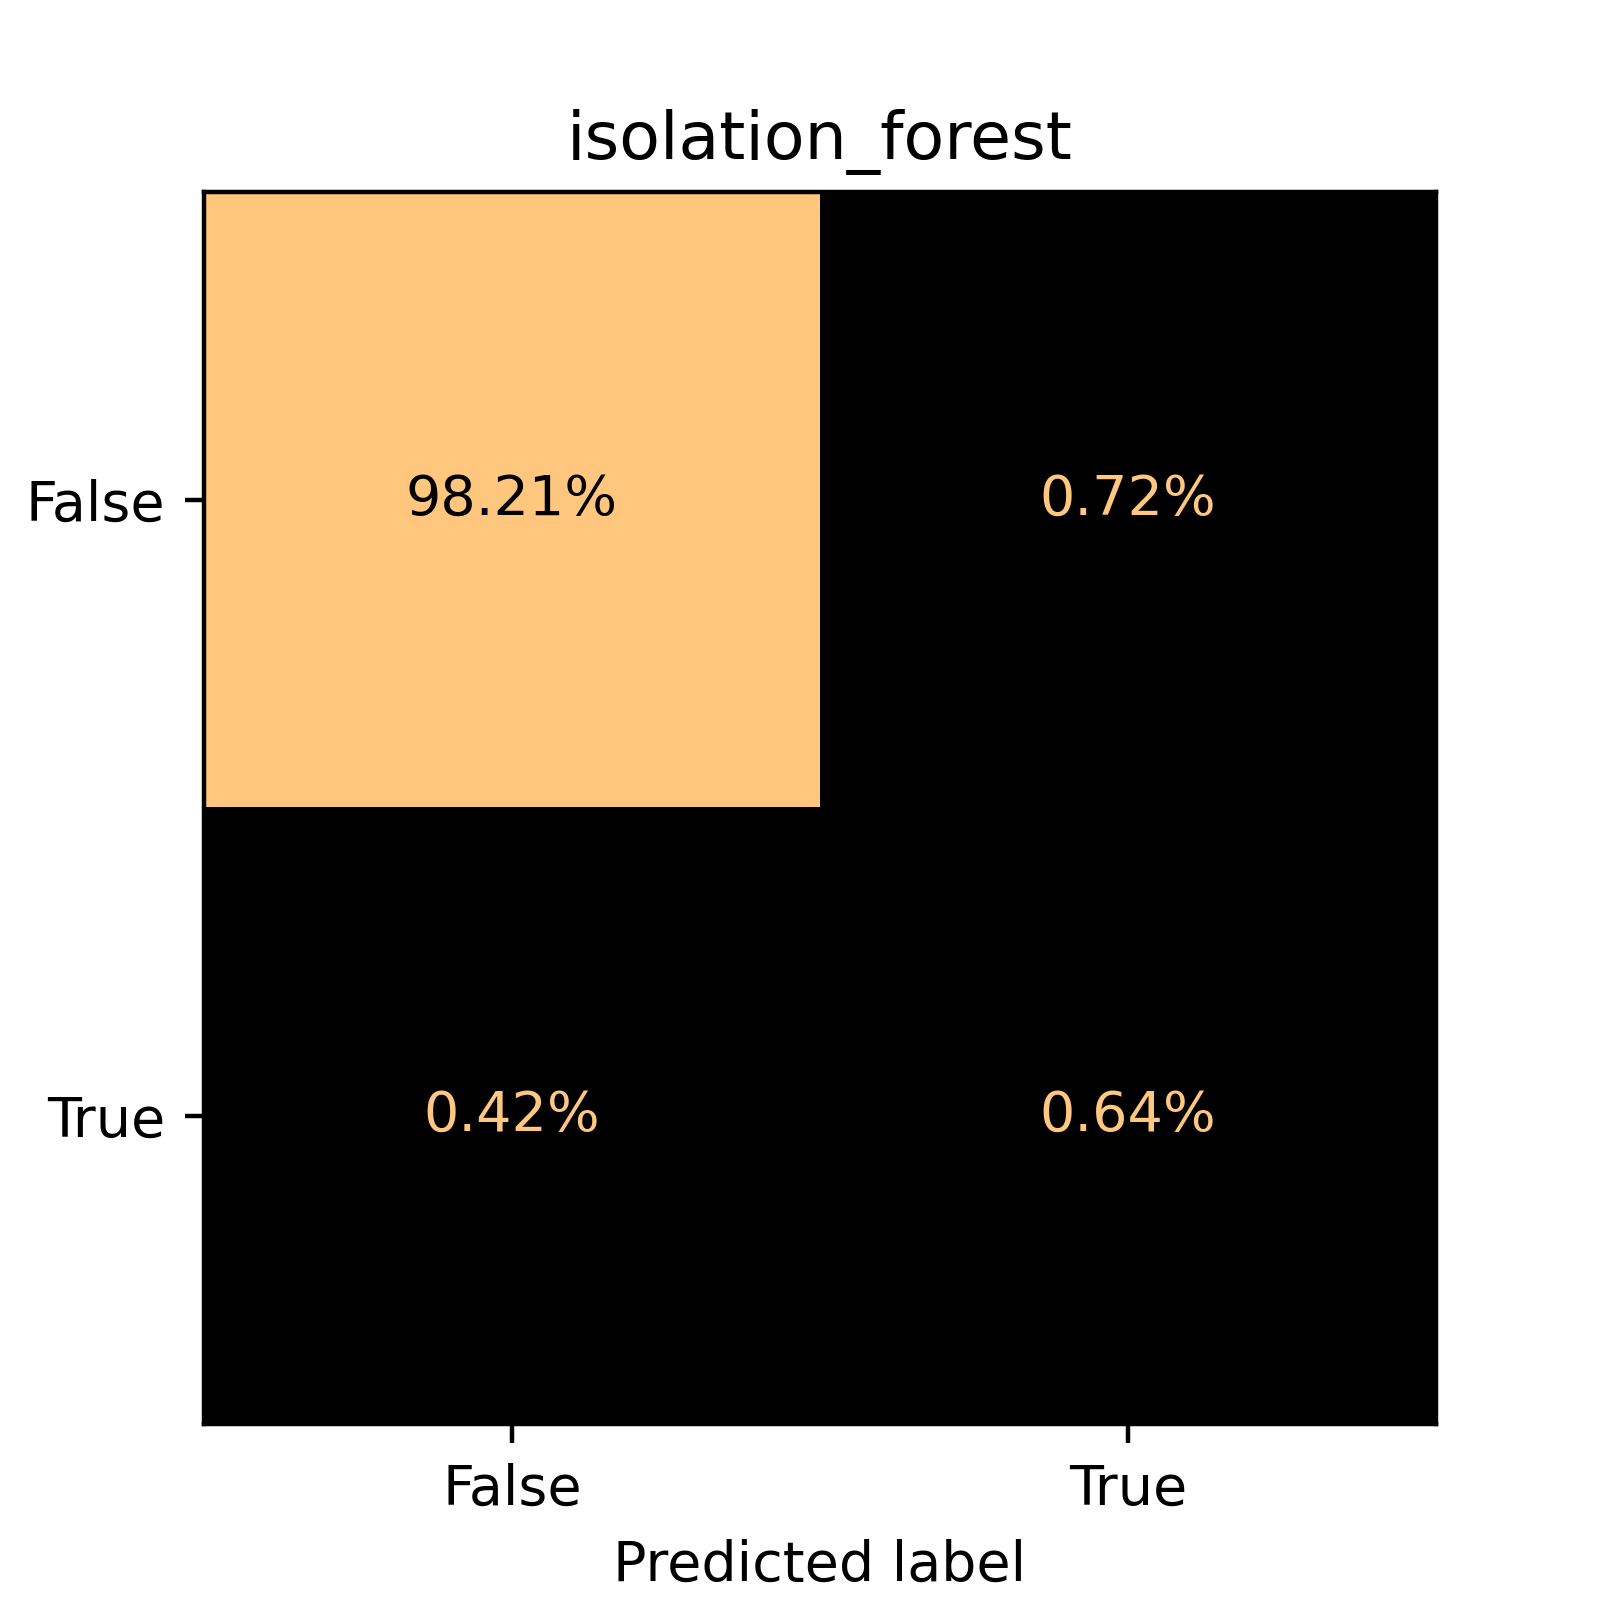
\includegraphics[width=\textwidth]{./results/resnet50_vgg19/20230514_213740_isolation_forest_cm.png}
    \end{subfigure}
    \caption{Confusion Matrices of the ResNet50 Encoder}
    \label{fig:resnet50_cm}
\end{figure}